\documentclass[a4paper,12pt]{report}
\usepackage[utf8]{inputenc}
\usepackage[francais]{babel}
\usepackage{fancyhdr}
\usepackage{graphicx}
\usepackage{tikz}
\usetikzlibrary{calc}
\usepackage{listings}
\usepackage{xcolor}
\definecolor{grey}{rgb}{0.9,0.9,0.9}
\usepackage{titlesec}
\usepackage{verbatim}
\usepackage{listings}
\usepackage{textcomp}
\usepackage{hyperref}
\usepackage{longtable}
\usepackage{colortbl}
\usepackage{amssymb}


\frenchbsetup{StandardLists=true}
\newcommand{\marge}{18mm}
\usepackage[left=\marge,right=\marge,top=\marge,bottom=\marge]{geometry}
\pagestyle{fancy}
\setlength{\headheight}{14pt}
\chead{
  \textbf{Binôme :} Douaille Erwan 
    \hspace{2em}
  \textbf{Groupe :} M2 Info IVI}
\renewcommand{\headrulewidth}{1pt}
\linespread{1}
\setlength{\columnseprule}{0.2pt}
\definecolor{javakeyword}{rgb}{0,0,0.5}
\definecolor{javastring}{rgb}{0,0.5,0}
\definecolor{javacomment}{rgb}{0.5,0.5,0.5}
\lstdefinestyle{java}{
   language=Java, basicstyle=\footnotesize,       % the size of the fonts that are used for the code
  numbers=left,                   % where to put the line-numbers
  numberstyle=\tiny\color{gray},  % the style that is used for the line-numbers
  stepnumber=1,                   % the step between two line-numbers. If it's 1, each line
                                  % will be numbered
  numbersep=5pt,                  % how far the line-numbers are from the code
  backgroundcolor=\color{white},  % choose the background color. You must add \usepackage{color}
  showspaces=false,               % show spaces adding particular underscores
  showstringspaces=false,         % underline spaces within strings
  showtabs=false,                 % show tabs within strings adding particular underscores
  frame=single,                   % adds a frame around the code
  rulecolor=\color{black},        % if not set, the frame-color may be changed on line-breaks within not-black text (e.g. commens (green here))
  tabsize=2,                      % sets default tabsize to 2 spaces
  captionpos=b,                   % sets the caption-position to bottom
  breaklines=true,                % sets automatic line breaking
  breakatwhitespace=false,        % sets if automatic breaks should only happen at whitespace
  title=\lstname,                 % show the filename of files included with \lstinputlisting;
   stringstyle=\color{javastring},
   keywordstyle=\color{javakeyword}\ttfamily\textbf,
   commentstyle=\color{javacomment}\ttfamily\textit
 }
 

\begin{document}



\makeatletter
\begin{titlepage}
\centering
\vspace{-10em}
{\LARGE \textbf{\textsc{Rapport de Projet RVI}}}\\
\vspace{3em}

\includegraphics[scale=0.6]{image/thalassa.png}\\
\vspace{3em}
{\LARGE \textsc{Projet Thalassa: simulation de plongée sous-marine}}\\

\vspace{8em}
Par\\
\vspace{1em}
{\LARGE \@author}\\

\vspace{2em}



\begin{tikzpicture}[remember picture,overlay]

\node [below left,xshift=-1cm, yshift=4cm] at (current page.south east){
\includegraphics[scale=0.6]{image/ustl1.png}};

\end{tikzpicture}
\end{titlepage}
\makeatother

\sloppy

\setcounter{page}{1} 
\newpage

\section*{Introduction}

Le but de ce TP est de nous faire découvrir la modification d'images couleur. Pour cela nous utiliserons les composantes HSB (Teinte, Saturation et Luminance) avec lesquelles nous observerons la perte d'informations et les conséquences de la modification de ces composantes.

\section*{Exercice 1}

\subsection*{Question 1}

En comparant ces deux images on observe que l'image de droite est plus lumineuse que l'image de gauche.  En observant l'image dans l'espace couleur on remarque que les pixels de l'image sombre sont moins élevés sur l'axe central. 

\begin{figure}[!ht]
	\center
	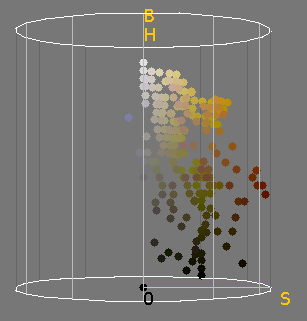
\includegraphics[scale=0.5]{image/q1_1.png}
	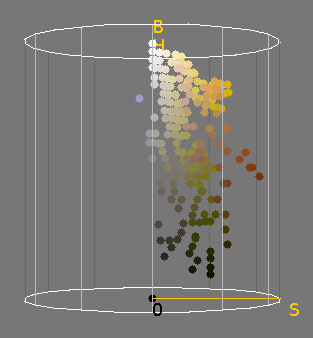
\includegraphics[scale=0.48]{image/q1_2.png}
	\caption{image gauche: \textit{it1$\_$72pp$\_$sombre}, image droite: \textit{it1$\_$72pp}}
\end{figure} 
 
Cette différence est liée au facteur \textit{Brightness}, donc de luminosité, visible dans l'espace de couleur \textit{HSB} (teinte, saturation et lumière). En manipulant les données, on peut retrouver l'image de droite grâce à l'image de gauche en diminuant \textit{Brightness} de 30. 

\newpage

\subsection*{Question 2}
 
\begin{lstlisting}[style=Java,caption={Code question 2},label=lst:question 2]
macro "augmentation_luminance" {
	image = getImageID();
	valeur = getNumber ("quelle augmentation (absolue) de luminance",valeur);
	setBatchMode(true);
	W = getWidth();
	H = getHeight();
	run("Duplicate...", "title=luminance modifiee");
	image_luminance_aug = getImageID();
	for (j=0; j<H; j++) {
		for (i=0; i<W; i++) {
			selectImage (image);
			couleur_avant = getPixel(i,j);
			R_avant = (couleur_avant & 0xff0000) >> 16;
			G_avant = (couleur_avant & 0x00ff00) >> 8;
			B_avant = (couleur_avant & 0x0000ff) ;
			R_apres = R_avant+valeur;// fonction de R_avant ;
			G_apres = G_avant+valeur;// fonction de G_avant ;
			B_apres = B_avant+valeur;// fonction de B_avant ;
			couleur_apres = ((R_apres & 0xff ) << 16) + ((G_apres & 0xff) << 8) + B_apres & 0xff;
			selectImage (image_luminance_aug);
			setPixel(i,j,couleur_apres);
		}
	}
	setBatchMode(false);
}
\end{lstlisting}

Dans cette macro, nous récupérons une valeur de luminosité que nous appliquerons. Ensuite nous parcourons tout les pixels de l'image. Nous récupérons les composantes \textit{RGB} et nous ajoutons cette valeur de luminosité que nous sauvegarderons dans une autre image.

Pour vérifier que l'image obtenue est correcte il est possible de faire une soustraction de l'image obtenue par l'image originale.

\begin{figure}[!ht]
	\center
	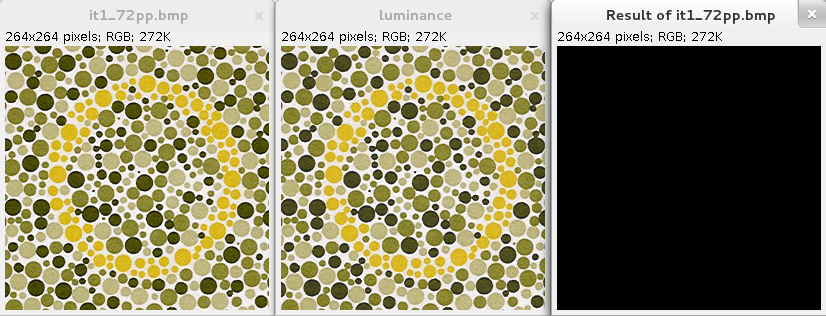
\includegraphics[scale=0.5]{image/q2.png}
\end{figure} 

On obtient une image noir ce qui confirme que l'image obtenue est correcte.

\newpage

\subsection*{Question 3 et 4}

Pour les images \textit{it1}, \textit{it2} et \textit{it3} nous avons respectivement trouvé comme valeur, ayant le meilleur résultat, 30, 41 et 60.

Voici un aperçu des images obtenues:

\begin{figure}[!ht]
	\center
	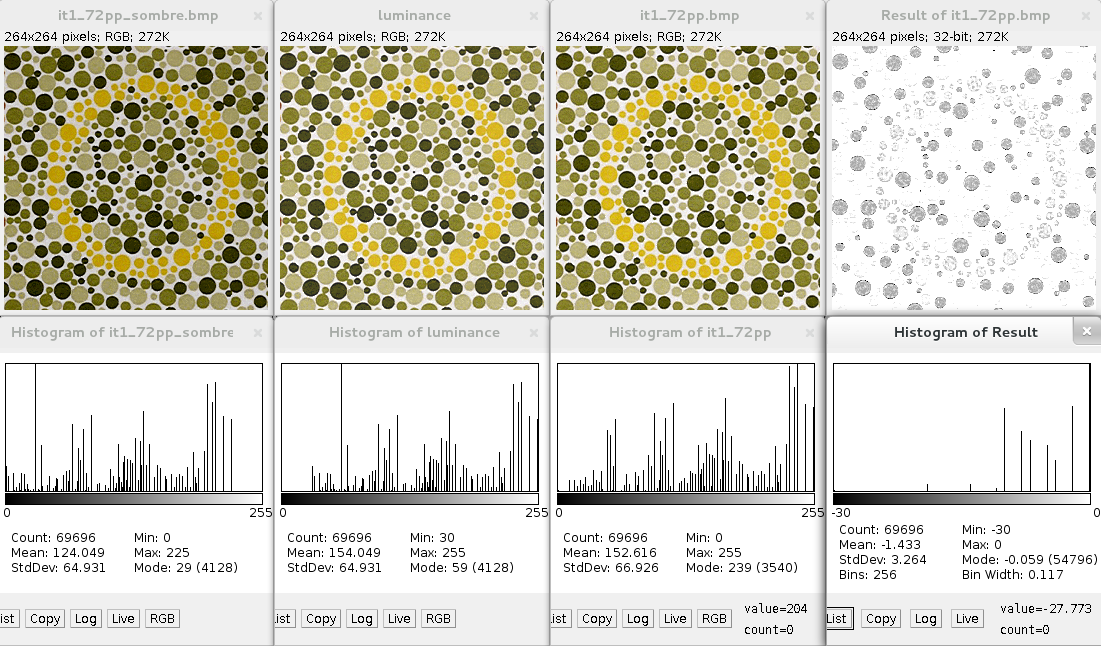
\includegraphics[scale=0.32]{image/q3-1.png}
\end{figure} 

\begin{figure}[!ht]
	\center	
	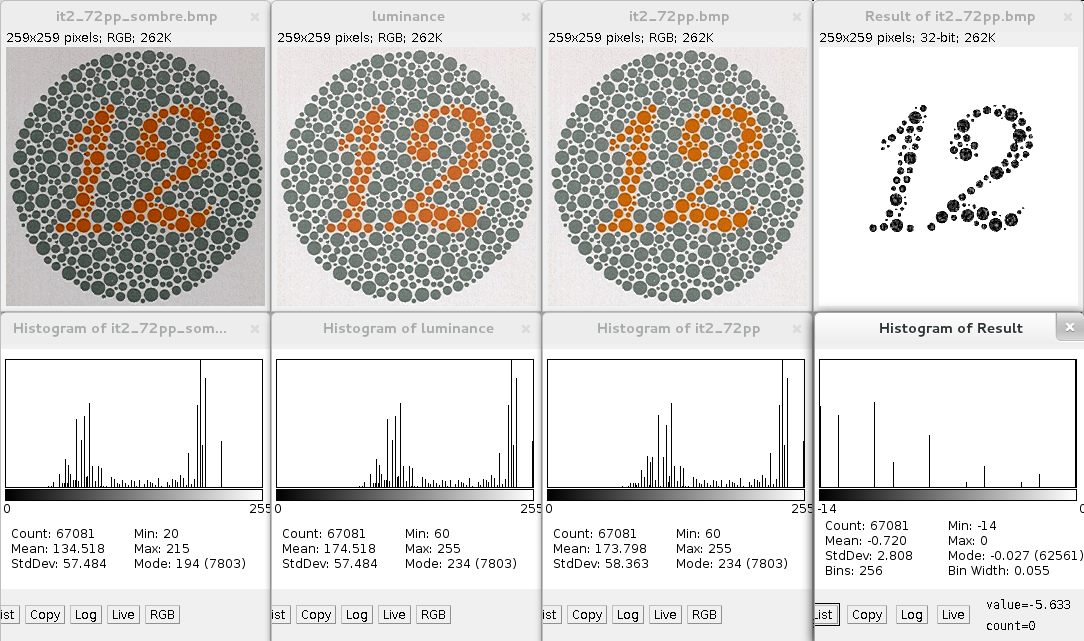
\includegraphics[scale=0.32]{image/q3-2.png}
	
	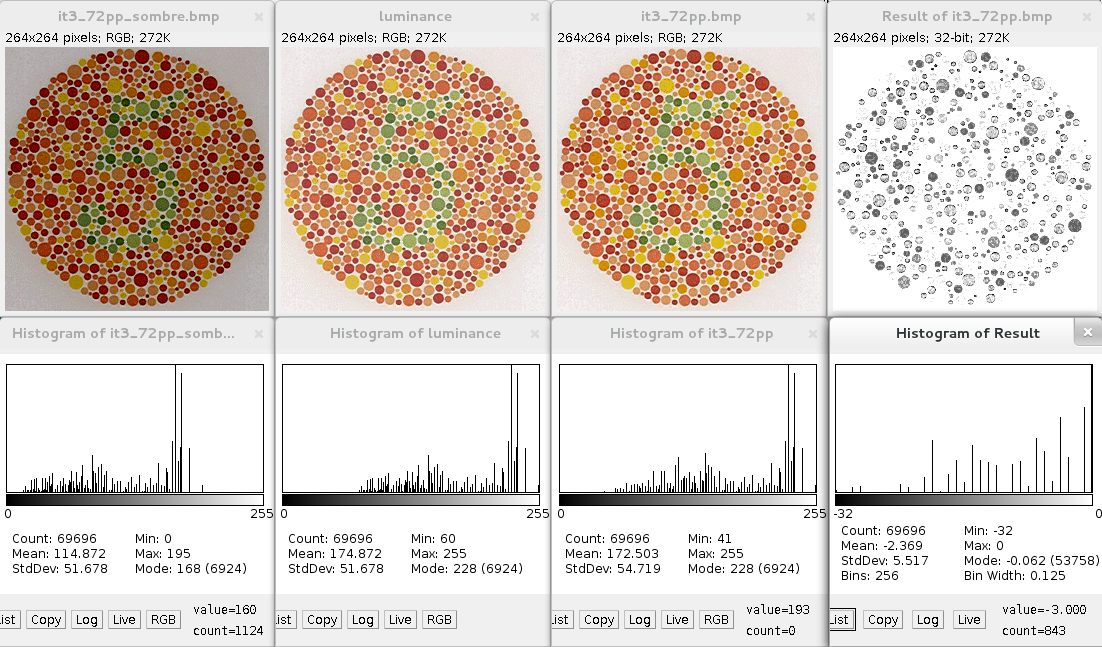
\includegraphics[scale=0.32]{image/q3-3.png}
\end{figure} 

En observant les histogrammes et images résultantes on s'aperçoit que les images résultantes diffèrent des images originales.

Cette différence est dûe au passage en 32 bit. De l'information a été perdue pour passer de l'image d'origine à l'image sombre. En appliquant par exemple une luminance de 30 on ne comble pas ce manque d'information. On s'approche donc de l'image originale sans pour autant obtenir une parfaite reconstruction.

\section*{Exercice 2}

\subsection*{Question 1}

La différence entre \textit{it2$\_$72pp} et \textit{it2$\_$72$\_$gris} est que la première image est en couleur et la seconde est en noir et blanc.

Voici un aperçu de la distribution des couleurs:

\begin{figure}[!ht]
	\center
	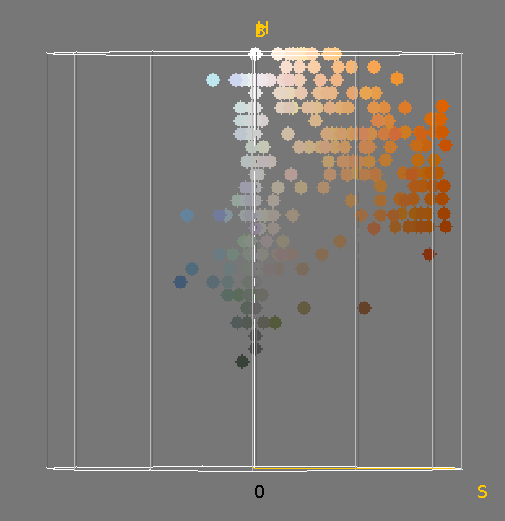
\includegraphics[scale=0.4]{image/E2q1-2.png}
	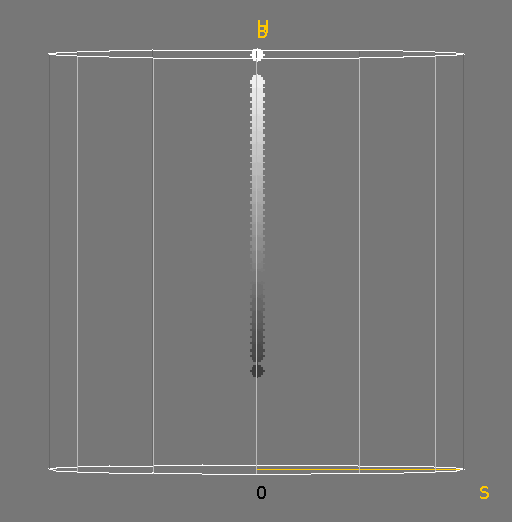
\includegraphics[scale=0.4]{image/E2q1-1.png}	
	\caption{image gauche: \textit{it2$\_$72pp}, image droite: \textit{it2$\_$72$\_$gris}}
\end{figure} 

Dans la pratique il faut imaginer que les pixels couleurs sont plaqués sur l'axe central, pour obtenir l'image noir et blanc.	

\subsection*{Question 2} 

Non, il sera impossible de retrouver une image couleur à partir de l'image en niveaux de gris. C'est dûe au fait que les informations RGB ont été perdues lors du passage en niveaux de gris.

\subsection*{Question 3}

\begin{figure}[!ht]
	\center
	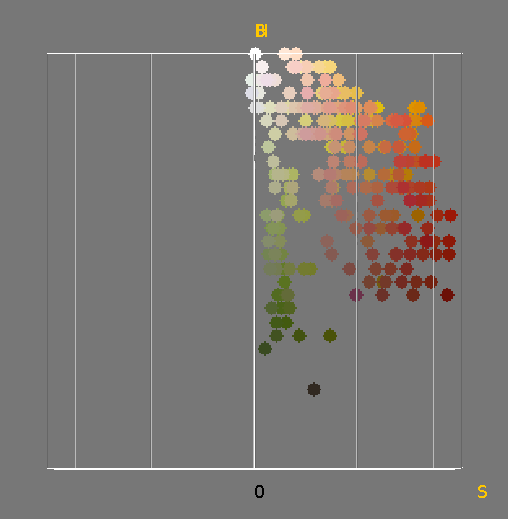
\includegraphics[scale=0.4]{image/E2q2-1.png}	
	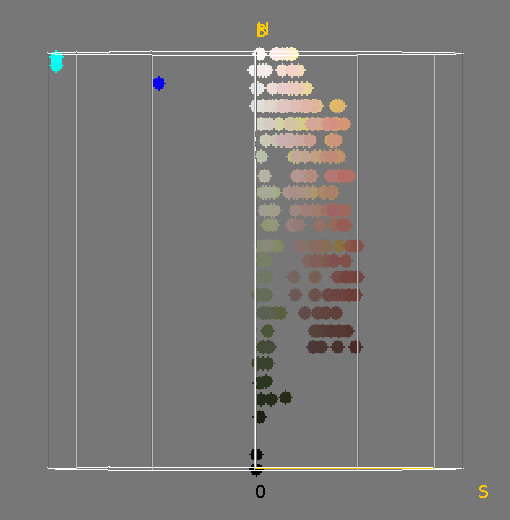
\includegraphics[scale=0.4]{image/E2q2-2.png}
	\caption{image gauche: \textit{it3$\_$72pp}, image droite: \textit{it3$\_$72$\_$saturation$\_$faible}}
\end{figure} 

La saturation, autrement dit chromaticité, correspond à l'intensité de la couleur. On observe sur l'image de droite que l'intensité de la couleur est moin importante. Les pixels sont plus proches de l'axe central et donc peu élevé sur l'axe chromatique. On observe que réduire la saturation à son maximum permet d'obtenir une image en niveaux de gris, comme ce qui a été fait lors de la question 1.

\newpage

\subsection*{Question 4}

Voici le code principale de la macro permettant d'augmenter la saturation.
\begin{lstlisting}[style=Java,caption={Code question 4},label=lst:question 4]
open("/home/m2ivi/douaille/VISA/tp_couleur/it3_72pp_saturation_faible.bmp");
run("Color Space Converter", "from=RGB to=HSB white=D65");
run("Split Channels");
selectWindow("it3_72pp_saturation_faible.bmp (HSB) (green)");
run("Multiply...", "value=1.250");
run("Merge Channels...", "red=[it3_72pp_saturation_faible.bmp (HSB) (red)] green=[it3_72pp_saturation_faible.bmp (HSB) (green)] blue=[it3_72pp_saturation_faible.bmp (HSB) (blue)] gray=*None*");
run("Color Space Converter", "from=HSB to=RGB white=D65");
\end{lstlisting}

Dans ce code est effectué exactement ce qui est demandé dans l'énoncé. On sélectionne la fenêtre verte car dans le système HSB, la saturation est représentée par la fenêtre verte (Saturation). On a ensuite augmenté la valeur de saturation pour obtenir l'image suivante:

\begin{figure}[!ht]
	\center
	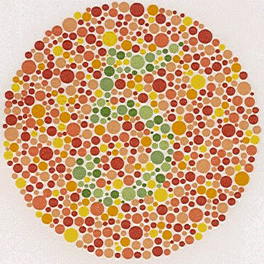
\includegraphics[scale=0.4]{image/E2-41.png}	
	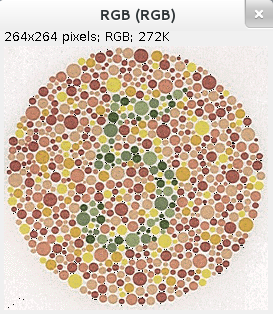
\includegraphics[scale=0.4]{image/E2-4.png}	
	\caption{image gauche: \textit{image original}, image droite: \textit{image obtenue}}
\end{figure} 

Le problème de cette macro est qu'elle applique à l'ensemble des pixels une saturation plus importante alors que certain de ces pixels ont déjà une valeur correcte. Cette macro augmente la saturation globale ce qui aura pour résultat d'obtenir une image plus colorée que l'image de base dans le cas d'une correction se rapprochant de la saturation originale. On peut remarquer que certains pixels blanc sont devenus colorés.

\section*{Exercice 3}

\subsection*{Question 1}

Voici le code principale de la macro permettant d'augmenter la teinte.
\begin{lstlisting}[style=Java,caption={Code question 1},label=lst:question 1]
open("/home/m2ivi/douaille/VISA/tp_couleur/it3_72pp.bmp");
run("Color Space Converter", "from=RGB to=HSB white=D65");
run("Split Channels");
selectWindow("it3_72pp.bmp (HSB) (red)");
run("Add...", "value=50");
run("Merge Channels...", "red=[it3_72pp.bmp (HSB) (red)] green=[it3_72pp.bmp (HSB) (green)] blue=[it3_72pp.bmp (HSB) (blue)] gray=*None*");
run("Color Space Converter", "from=HSB to=RGB white=D65");
\end{lstlisting}

Dans ce code est effectué exactement ce qui est demandé dans l'énoncé. On sélectionne la fenêtre rouge car dans le système HSB, la teinte est représenté par la fenêtre rouge (Hue). On a ensuite augmenté la valeur la teinte pour obtenir l'image suivante:

\begin{figure}[!ht]
	\center
	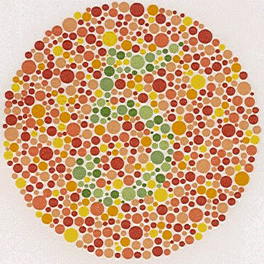
\includegraphics[scale=0.5]{image/E2-41.png}	
	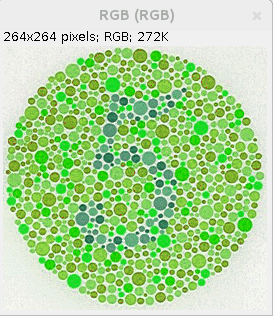
\includegraphics[scale=0.5]{image/E3-1.png}	
	\caption{image gauche: \textit{image original}, image droite: \textit{image obtenue}}
\end{figure} 

Grâce à cette macro je peux maintenant lire le 5 !
La teinte agit sur la couleur.

\section*{Conclusion}

Dans ce TP nous avons observé comment fonctionnait le modèle HSB (Hue, Saturation and Brightness) en jouant avec les différentes composantes. Nous avons pu constater que la perte d'informations était présente lorsque l'on changeait la saturation ou la luminance et que à partir de ces nouvelles images nous souhaitions obtenir les images originales.

\end{document}